\subsection{Introduction}

Small molecules are excellent tools for probing biological functions and continue to be the cornerstone of pharmaceutical companies. Synthetic chemical compounds present a complex structural code that, for the most part, has not been explored by the principles of natural evolution. Many pharmacological compounds are imperfect human inventions with sub-optimal bioactivities that lack a clear connection to their chemical structure. Often, the only way to approach the biological characterization of a compound is to assume it will have comparable bioactivities to compounds with similar chemical properties. The so-called ‘similarity principle’ has been the driving force of drug discovery efforts\cite{kumar_advances_2018}, and the measurement of compound similarities lays behind most of the approaches used to explore the vast drug-like chemical space (estimated in the range of 10\textsuperscript{33}-10\textsuperscript{66} molecules\cite{polishchuk_estimation_2013, bohacek_art_1996}). To assess such similarities, molecules are usually characterized using numerical fingerprints or descriptors\cite{cereto-massague_molecular_2015}, which encapsulate their main topological and physicochemical properties representing them in a format amenable for computational applications (e.g. QSAR\cite{yang_concepts_2022}).

In the last years, the extensive gathering and release of bioactivity data have shown that the similarity principle applies beyond standard chemical features, reaching to functional properties. For instance, small molecules that show similar sensitivity profiles across human tumor cell-lines or drugs that cause comparable side effects in patients tend to share mechanisms of action (MoA), even when they are structurally dissimilar\cite{holbeck_analysis_2010, seashore-ludlow_harnessing_2015, campillos_drug_2008}. Thus, bioactivity similarities offer an alternative means to functionally characterize small molecules, potentially providing insights closer to clinical observations and surpassing what is expected from merely inspecting chemical analogues\cite{petrone_rethinking_2012}.

%%%%%%%%%%%%%%%%
%%% FIGURE 1 %%%
%%%%%%%%%%%%%%%%


\begin{figure}[t!]
  \centering
  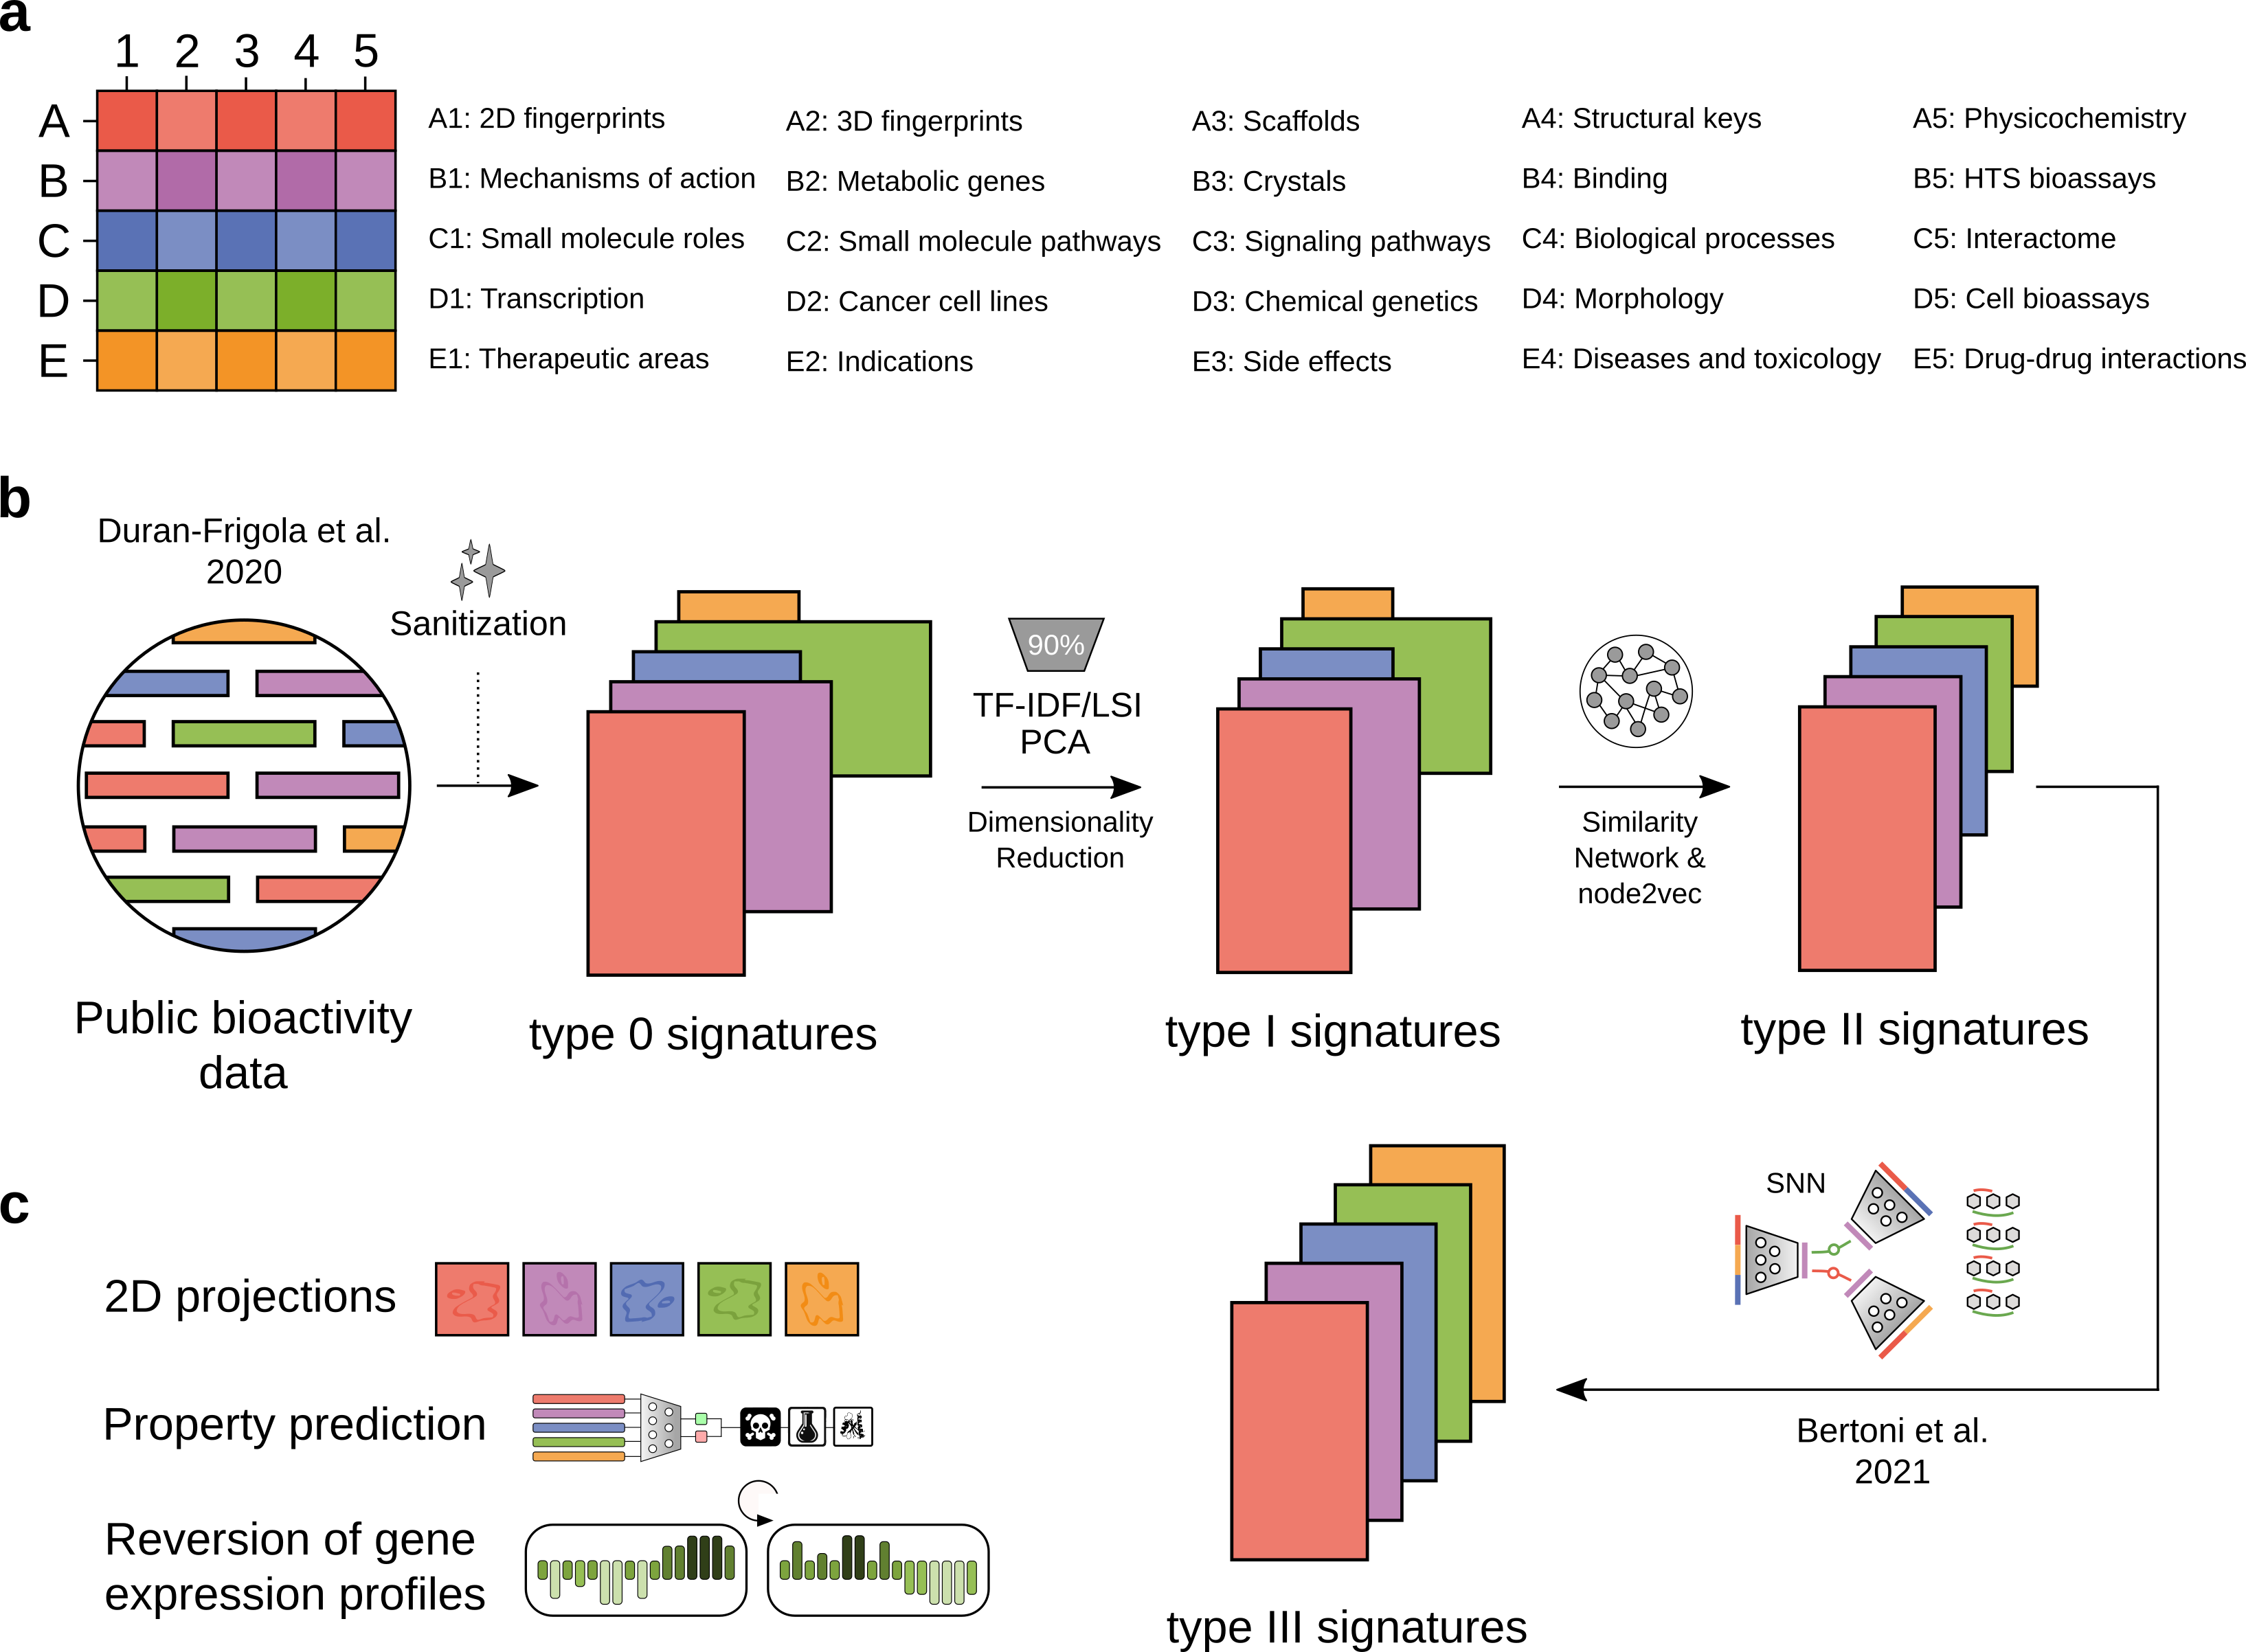
\includegraphics[width=\linewidth]{figures/Protocols/Main/CC.png}
  \caption{
    \textbf{CC Overview.} 
    \textbf{a)} Organization of the 25 CC spaces.
    \textbf{b)} Computational pipeline to build the CC and procedure to integrate bioactivity data in the CC universe. In brief, bioactivity data is sanitized (type 0 signatures), compressed (type I signatures), harmonized (type II signatures) and integrated with all the other data within the CC (type III signatures).
    \textbf{c)} Compound signatures are used in a variety of tasks, such as the characterization and visualization of large small molecule libraries, the prediction of multiple properties (e.g. toxicity, physicochemical properties, protein binding, etc.) and the reversion of gene expression profiles associated with specific disease states, among many others. 
    \rule[0ex]{\textwidth}{0.5pt}
  }
  \label{Protocols_Fig1}
\end{figure}



\phantomsection
\subsubsection{The Chemical Checker}

We recently developed the Chemical Checker (CC, Fig \ref{Protocols_Fig1}a), the largest collection to date of processed, harmonized and integrated bioactivity signatures for over 1 million compounds, whose biological effects had been experimentally determined\cite{duran-frigola_extending_2020}. Following the way in which we understand drug action, we organized data in 25 bioactivity spaces grouped in 5 levels of increasing biological complexity: from physicochemical and structural properties of small molecules (A) to the clinical effects they exert in human patients (E). In between, we collect the set of biological targets they bind (B), the perturbations they trigger in biological pathways (C) and the phenotypic effects they induce in cell-based assays (D). Unfortunately, bioactivity data become scarcer and more difficult to obtain as biological complexity increases (i.e. we have direct protein-binding data for \textasciitilde630k small molecules but only \textasciitilde6k compounds are annotated with clinical indications), meaning that bioactivity information remains limited for poorly characterized compounds. To address this problem, we developed a collection of deep neural networks to infer CC bioactivity signatures for any compound of interest\cite{bertoni_bioactivity_2021, comajuncosa-creus_stereochemically-aware_2024}, based on the observation that the different bioactivity spaces are not completely orthogonal, and thus similarities of a given bioactivity type (e.g. targets) can be transferred to other data kinds (e.g. therapeutic indications). Moreover, we showed that the inferred bioactivity signatures are useful to navigate the chemical space in a biologically relevant manner and improve the performance of biophysics and physiology activity prediction activities with respect to chemistry-only based classifiers. In general, we believe that bioactivity signatures associated to small molecules have the power to reintroduce the biological complexity at the early stages of the drug discovery process, overcoming some of the problems associated with target-based approaches. For instance, using CC signatures, we were able to identify three compounds able to revert transcriptional signatures related to Alzheimer’s disease \textit{in vitro} and \textit{in vivo}\cite{pauls}. Moreover, using CRISPR-Cas9 and shRNA perturbation experiments as templates, we also identified several small molecules that mimicked the phenotypic effects of biodrugs (e.g. daclizumab, ustekizumab, cetuximab, etc.), often through a different MoA that did not directly modulate the activity of their primary targets (e.g. IL-2R, IL-12 and EGFR)\cite{duran-frigola_extending_2020}, and targeted cancer proteins though to be undruggable\cite{bertoni_bioactivity_2021}.


The original 25 CC bioactivity spaces (Fig \ref{Protocols_Fig1}a) comprise data retrieved from publicly available databases at the time that were processed through a unified data curation and integration pipeline. Compound bioactivities are expressed in a vector-like format (i.e. signatures) and organized in increasing levels of abstraction: from raw data accounting for explicit knowledge (type 0 signatures) to inferred representations leveraging known bioactivity patterns (type III signatures). However, in the last years, new large-scale assays to capture biological responses to small molecule perturbations, and more efficient computational strategies to process them, are constantly appearing\cite{anglada-girotto_combining_2022, mitchell_proteome-wide_2023, offensperger_large-scale_2024}. Besides, there is an ever-growing number of laboratories and biotechnological companies that have their own in-house data and want to leverage it together with the bulk of known bioactivity information. Thus, in this manuscript, we present the complete computational protocol to generate novel bioactivity spaces and signatures, describing the main steps needed to leverage diverse bioactivity data with the Chemical Checker (type 0, type I, type II and type III signatures) using the predefined data curation and integration pipeline.

\phantomsection
\subsubsection{Overview of the Chemical Checker data integration pipeline}

The main input for the CC integration pipeline is a bioactivity data matrix encompassing compounds (rows, e.g. InChIKeys) and biological features (columns, unique strings: e.g. protein targets (B4), mechanisms of action (B1), clinical side effects (E3), etc.). Data might be categorical (e.g. binary), discrete or continuous.

-- Type 0 signatures